\section{Fundamentos del Framework}
En la sección~\ref{sec:petri_concurrency_monitor_intro} se propone utilizar RdP
como la lógica secuencial de un sistema concurrente. Para logralo, se
implementó el monitor de petri por software descripto en la
sección~\ref{sec:java_petri_concurrency_monitor}.
Este monitor permite delegar la concurrencia y asincronismo del
sistema a una red de Petri \cite{TesisMicolini}. Un ejemplo de uso exitoso se
describe en \cite{Bentivegna-Ludemann}.

La utilización directa del monitor es engorrosa y genera un
alto grado de acoplamiento entre el software de usuario y la red de Petri
puesto que los eventos de la red quedan asociados directamente a los eventos del
mundo real que modela.
La principal desventaja de un sistema acoplado a la red de Petri está dada por la
reducción de la escalabilidad del sistema. Esto se debe a que una modificación
de la lógica, que conlleva una sustitución de la red, implica también un cambio
en el código del software. En consecuencia, dificulta el proceso de desarrollo y
su mantenibilidad. Otra desventaja es que impide la reutilización de redes de
Petri genéricas, útiles para resolver diferentes problemas de
características similares.

Un requerimiento importante de este proyecto consiste en la facilidad de uso.
Como se explicó en el párrafo anterior, la utilización del monitor en forma
directa presenta una complejidad elevada y favorece a la generación de errores,
ya que deben crearse todos los hilos de ejecución y deben programarse los disparos de
transición de forma manual en el código. Este problema se manifiesta, por
ejemplo, en soluciones como CodeGen \cite{codegen}.
Ante un cambio en la Red de Petri deben modificarse algunos o todos los
disparos de transición distribuidos a lo largo del código. En caso de un error
en esta tarea, se genera una sincronización incorrecta de los hilos.

A su vez, para desacoplar las acciones que debe realizar el sistema de los
eventos, es necesario incorporar una entidad encargada de manejar y ejecutar
dichas acciones.

Como resultado de este análisis, se llegó a la conclusión de que es necesario
embeber el monitor de Petri en un framework que se encargue de desacoplar el
código de usuario de la lógica de disparos.
Una conclusión de similares características se desprende de
\cite{Bentivegna-Ludemann}, donde los autores expresan: ``La debilidad
encontrada en el proceso de elaboración del software, es que resultó
problemático vincular los hilos con las transiciones de la RdP. Esto se debe a
que entre las acciones y las transiciones no existe una capa de abstracción
para mapear las mismas.
Por lo cual, queda en evidencia que es necesaria la existencia de un framework
para automatizar y facilitar la vinculación entre eventos, acciones y
transiciones.''


\section{Sincronización por Red de Petri a través de Eventos}
\label{sec:sincronizacion_RdP_por_eventos}
Los sistemas a desarrollar utilizando el monitor descripto en la
sección~\ref{sec:java_petri_concurrency_monitor}, son programas de software que
intercambian eventos con la red de Petri y con su entorno físico.

\begin{figure}[h]
	\centering
	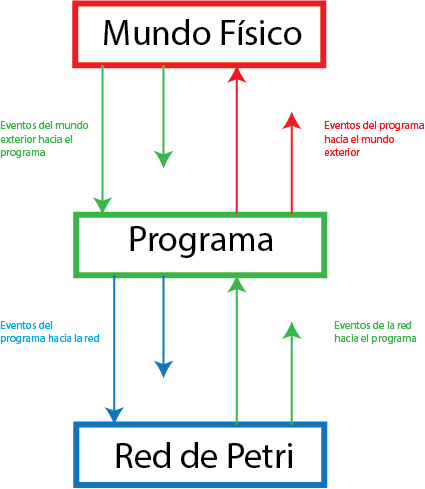
\includegraphics[width=75mm]{eventos_petri-programa-mundo}
	\caption{Intercambio de eventos en un programa sincronizado por Red de Petri}
	\label{fig:eventos_petri-programa-mundo}
\end{figure}

El programa tiene la posibilidad de acceder a hardware del mundo físico, ya sea
para realizar una acción (por ejemplo utilizando actuadores) o  para obtener
eventos del mundo exterior y comunicarlos a la red de Petri (por ejemplo con
sensores).

La red toma los eventos del mundo exterior y, dependiendo de las condiciones del
problema y del estado global, calcula los eventos hacia el programa.
La red es un procesador de eventos. \cite{TesisMicolini}\cite{chimp}

Este concepto se amplía en la sección Eventos Físicos y Eventos
Lógicos de \cite{chimp}. En esta sección se distingue la existencia de los dos
tipos de eventos mencionados, y se los define como:
  \begin{itemize}
    \item Eventos Lógicos: eventos que son comprensibles por el monitor de
    redes de Petri, y están inherentemente asociados a transiciones de la red
    misma y sus colas.
    \item Eventos Físicos: suceden en el mundo físico y representan sucesos del
    dominio del problema. Están conectados con el software.
  \end{itemize}

Tras la incorporación del concepto de eventos lógicos y físicos, en \cite{chimp}
se propone un diagrama de arquitectura de alto nivel como el de la
Figura~\ref{fig:eventos_fisicos-logicos}.

\begin{figure}[h]
	\centering
	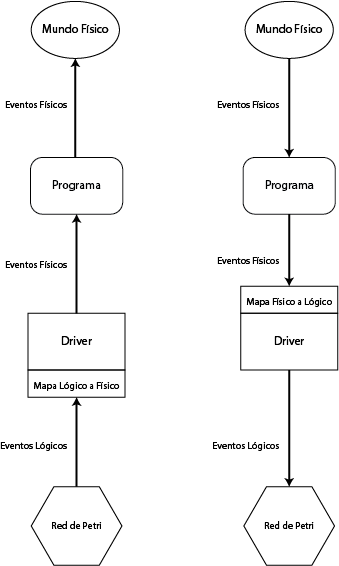
\includegraphics[width=75mm]{eventos_fisicos-logicos}
	\caption{Arquitectura con Eventos Físicos y Lógicos}
	\label{fig:eventos_fisicos-logicos}
\end{figure}

Los eventos físicos representados en la
Figura~\ref{fig:eventos_fisicos-logicos} abarcan dos tipos de eventos. Uno de
ellos está efectivamente relacionado con el hardware o software externos al
sistema (mundo físico). El otro tipo de eventos está relacionado con el manejo
de las acciones que van a realizar dichos elementos del mundo exterior, el cual
se ejecuta a través del software del sistema.
Por este motivo se determinó que la clasificación de los
eventos en dos tipos no es suficiente para explicar la comunicación en un
sistema de estas características. 

A partir de lo expuesto en el párrafo previo, se modifica la clasificación
de eventos existente:

\begin{itemize}
    \item Eventos Lógicos: Conserva la definición descripta previamente. Este
    tipo de eventos se comunica utilizando las interfaces proporcionadas por el
    monitor de redes de Petri.
    \item Eventos Físicos: suceden en el mundo físico y representan sucesos del
    dominio del problema. Este tipo de eventos se comunican a través de las
    interfaces que expone el elemento del mundo exterior y las interfaces que
    ofrece el lenguaje de programación utilizado para desarrollar el software.
    Por ejemplo pueden comunicarse a través de Event Listeners, mecanismos
    de IPC, Sockets, Serial, Bluetooth, etc.
    \item Eventos de Acción: Evento intermedio
    entre los eventos físicos y lógicos. Este tipo de eventos es manejado
    por el framework durante la inicialización del sistema. Cumplen una función
    de abstracción entre las acciones de software y los eventos lógicos,
    necesaria para desacoplar la red de Petri del software y permitir la
    inversión de control descripta en la sección~\ref{sec:inversion_control}.
\end{itemize}

A partir de la nueva clasificación de los eventos del sistema emerge una nueva
arquitectura de alto nivel. A su vez emergen nuevos requerimientos, relacionados
con el requerimiento número 2 de la sección~\ref{sec:definicion_reqs}. A continuación
se listan los nuevos requerimientos:

\begin{itemize}
  \item El monitor de RdP debe manejar los eventos lógicos del sistema,
  mediante las interfaces de disparo y evaluación de guardas.
  \item El framework debe ofrecer interfaces para mapear eventos lógicos de una
  RdP a eventos de acción especificados por los usuarios.
\end{itemize}

\subsection{Arquitectura de alto nivel de \nombreFramework}
\label{sec:arquitectura_alto_nivel}
Un sistema informático consiste en una secuencia de acciones que se ejecutan
ante el cumplimiento de determinadas condiciones. Desde el punto de vista del
programa que analiza dichas condiciones, se las clasifica en síncronas y asíncronas.
  \begin{itemize}
	\item Síncronas: Están sicronizadas con la ejecución del programa. Se
	desencadenan en un momento específico, conocido de antemano.
	Por ejemplo, condiciones booleanas derivadas del estado del sistema que
	realizan cambios en el flujo de instrucciones del mismo (saltos
	condicionales).
	\item Asíncronas: Se desencadenan en cualquier momento, de forma independiente
	a la ejecución del programa. Por ejemplo, eventos provenientes del mundo
	exterior o mensajes entre procesos.
  \end{itemize}

El objetivo de este trabajo es implementar un framework dirigido por redes de
Petri para controlar la ejecución de todas aquellas acciones que respondan a
estos tipos de condiciones.
De esta forma, será el monitor de redes de Petri quien analice las condiciones y
explicite el estado del sistema. Así, es responsabilidad de la red:
\begin{itemize}
  \item Disparo de eventos provenientes de sistemas externos, que pueden llegar
  en cualquier instante de tiempo y sin un orden preestablecido. Los estados
  locales de la red se mantienen en causalidad de las acciones ejecutadas con
  anterioridad. El monitor es el encargado de mantener el estado lógico del
  sistema.
  
  \item Condiciones de sincronización para el ordenamiento de la ejecución de
  acciones en el tiempo. 
  
  \item Condiciones impuestas por el dominio del problema. El monitor es el
  encargado de impedir la ejecución de una acción hasta que la misma pueda ser
  realizada sin riesgos.
\end{itemize}

De acuerdo a lo estudiado en la sección~\ref{sec:inversion_control}, una
característica principal de un framework es la inversión de control. Por este
motivo, el diseño de la arquitectura del framework contempla el control del
flujo de ejecución del código de usuario.

\begin{figure}[H]
	\centering
	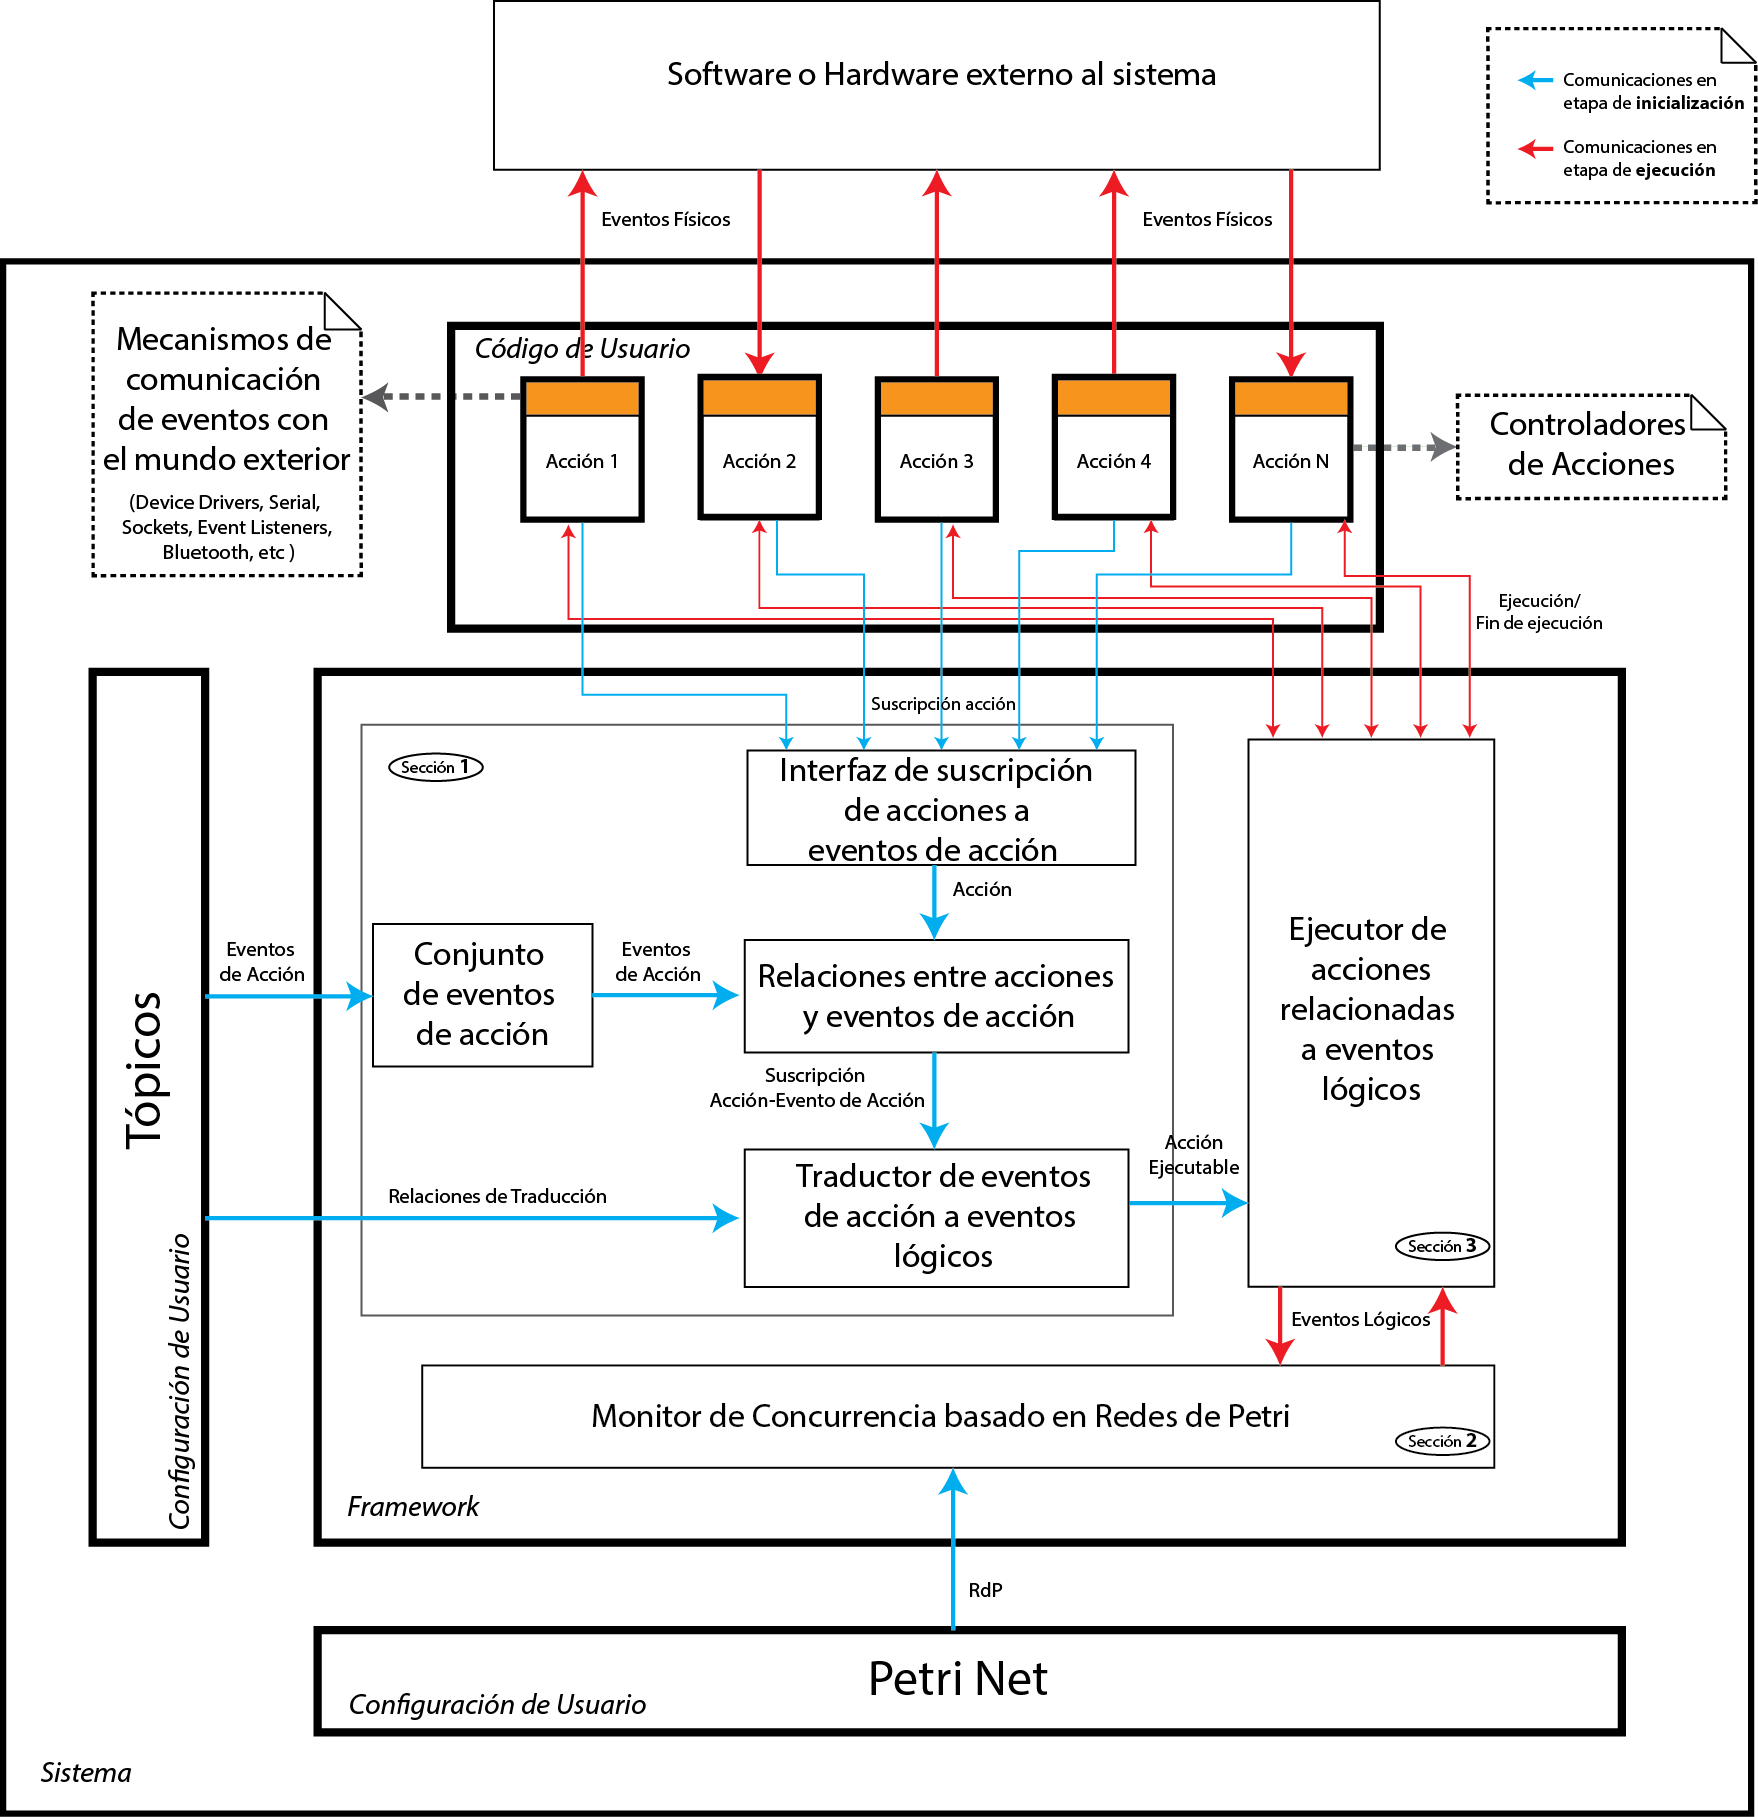
\includegraphics[width=0.9\textwidth]{arquitectura_framework}
	\caption{Diagrama de Arquitectura de Alto Nivel}
	\label{fig:arquitectura_petri-manejador-acciones-mundo}
\end{figure}

Como puede apreciarse en la
Figura~\ref{fig:arquitectura_petri-manejador-acciones-mundo}, \nombreFramework
Framework puede dividirse en tres partes a nivel de arquitectura:
\begin{enumerate}
  \item Un conjunto de módulos para la suscripción a eventos de acción (ver
  sección 1) encargado de:
  \begin{itemize}
    \item Ofrecer interfaces para definir los eventos de acción del sistema.
    \item Ofrecer interfaces para suscribir las acciones del sistema a los
    eventos de acción correspondientes.
    \item Ofrecer interfaces para definir las reglas de traducción entre eventos
    de acción y eventos lógicos.
    \item Encapsular las acciones junto a los eventos lógicos necesarios para su
    sincronización.
  \end{itemize}
\item Un monitor de redes de Petri (ver sección 2) cuyas responsabilidades son:
	\begin{itemize}
	  \item Brindar las interfaces para la incorporación del modelo de Red de Petri
	  del sistema, el cual contiene la definición de los eventos
	  lógicos.
	  \item Garantizar el cumplimiento de las condiciones de sincronización y
	  exclusión mutua de la concatenación de acciones.
	\end{itemize}
\item Un sistema ejecutor de las acciones definidas por el usuario (ver sección 3). 
  Se encarga de:
  \begin{itemize}
	  \item Intercambiar eventos lógicos con el monitor para asegurar la
	  sincronización y exclusión mutua en la ejecución de las acciones.
	  \item Ejecutar las acciones cuando las condiciones de ejecución
	  estén dadas.
	  \item Intercambiar eventos lógicos con el monitor para informar acerca de la
	  finalización de la ejecución de una acción.
	\end{itemize}
\end{enumerate}

Por su parte, el programa de usuario puede dividirse en:
\begin{enumerate}
  \item Una Red de Petri conteniendo el modelo de la lógica del sistema.
  \item Tópicos que contienen la definición de los eventos de acción y sus
  reglas de traducción a eventos lógicos.
  \item El código de usuario. Contiene todas las acciones de software
	concretas a realizar, con sus correspondientes suscripciones a eventos
	de acción. Dichas acciones pueden comunicarse con el mundo exterior. Por esta
	razón, \textbf{\emph{el manejo de los eventos físicos es responsabilidad del
	usuario}}.
\end{enumerate}

\begin{framed}
\textbf{Notas:} 
\begin{itemize}
\item Los controladores de acciones se ejecutan cuando el monitor de red de
Petri lo dispone. El monitor es el encargado de bloquear o liberar los hilos de una
acción de acuerdo a las condiciones de sincronizacion. Por otro lado, cuando una
acción finaliza, el sistema de ejecución se encarga de dar aviso al monitor.

\item La definición y el desarrollo de las acciones de software, y su
asociación a los eventos de acción correspondientes quedan a cargo del usuario
desarrollador. 

\item El usuario no decide en qué momento se ejecuta la acción, ya que
con el fin de lograr la inversión de control, dicha responsabilidad es otorgada
al monitor de redes de Petri.
\end{itemize}
\end{framed}